\documentclass[a4paper,12pt]{article}
\usepackage[colorlinks,linkcolor=black,urlcolor=black]{hyperref}
\usepackage{float}
\usepackage{mhchem}
\usepackage[table,xcdraw]{xcolor}
\usepackage{mathrsfs}
\usepackage{pdfpages}
\usepackage{enumerate}
\usepackage{amsmath}
\usepackage{setspace}
\usepackage{booktabs}
\usepackage{colortbl}
\usepackage{titlesec}
\usepackage{amssymb}
\usepackage{graphicx}
\usepackage{subfigure}
\usepackage{siunitx}
\usepackage{pdfpages}
\usepackage{wrapfig}
\usepackage{geometry}
\usepackage{indentfirst}
\usepackage{multirow} 
\usepackage{listings}
\usepackage{xcolor}
\usepackage{subfigure}
\usepackage{gensymb}
\usepackage[utf8]{inputenc}
\usepackage{listings}


\setlength{\parindent}{2em}
\renewcommand{\baselinestretch}{1.2}
\usepackage[greek,english]{babel} 
\geometry{left=2.8cm,right=2.8cm,top=2.2cm,bottom=2.2cm}


\lstset{
    numbers=left, 
    numberstyle= \tiny, 
    keywordstyle= \color{ blue!70},
    commentstyle= \color{red!50!green!50!blue!50}, 
    frame=shadowbox,
    rulesepcolor= \color{ red!20!green!20!blue!20} ,
    escapeinside=``,
    xleftmargin=2em,xrightmargin=2em, aboveskip=1em,
    framexleftmargin=2em,
    framexrightmargin=2em
} 
%\lstset{breaklines} 
\lstdefinelanguage[mips]{Assembler}{%
  % so listings can detect directives and register names
  alsoletter={.\$},
  % strings, characters, and comments
  morestring=[b]",
  morestring=[b]',
  morecomment=[l]\#,
  % instructions
  morekeywords={[1]abs,abs.d,abs.s,add,add.d,add.s,addi,addiu,addu,%
    and,andi,b,bc1f,bc1t,beq,beqz,bge,bgeu,bgez,bgezal,bgt,bgtu,%
    bgtz,ble,bleu,blez,blt,bltu,bltz,bltzal,bne,bnez,break,c.eq.d,%
    c.eq.s,c.le.d,c.le.s,c.lt.d,c.lt.s,ceil.w.d,ceil.w.s,clo,clz,%
    cvt.d.s,cvt.d.w,cvt.s.d,cvt.s.w,cvt.w.d,cvt.w.s,div,div.d,div.s,%
    divu,eret,floor.w.d,floor.w.s,j,jal,jalr,jr,l.d,l.s,la,lb,lbu,%
    ld,ldc1,lh,lhu,li,ll,lui,lw,lwc1,lwl,lwr,madd,maddu,mfc0,mfc1,%
    mfc1.d,mfhi,mflo,mov.d,mov.s,move,movf,movf.d,movf.s,movn,movn.d,%
    movn.s,movt,movt.d,movt.s,movz,movz.d,movz.s,msub,msubu,mtc0,mtc1,%
    mtc1.d,mthi,mtlo,mul,mul.d,mul.s,mulo,mulou,mult,multu,mulu,neg,%
    neg.d,neg.s,negu,nop,nor,not,or,ori,rem,remu,rol,ror,round.w.d,%
    round.w.s,s.d,s.s,sb,sc,sd,sdc1,seq,sge,sgeu,sgt,sgtu,sh,sle,%
    sleu,sll,sllv,slt,slti,sltiu,sltu,sne,sqrt.d,sqrt.s,sra,srav,srl,%
    srlv,sub,sub.d,sub.s,subi,subiu,subu,sw,swc1,swl,swr,syscall,teq,%
    teqi,tge,tgei,tgeiu,tgeu,tlt,tlti,tltiu,tltu,tne,tnei,trunc.w.d,%
    trunc.w.s,ulh,ulhu,ulw,ush,usw,xor,xori},
  % assembler directives
  morekeywords={[2].align,.ascii,.asciiz,.byte,.data,.double,.extern,%
    .float,.globl,.half,.kdata,.ktext,.set,.space,.text,.word},
  % register names
  morekeywords={[3]\$0,\$1,\$2,\$3,\$4,\$5,\$6,\$7,\$8,\$9,\$10,\$11,%
    \$12,\$13,\$14,\$15,\$16,\$17,\$18,\$19,\$20,\$21,\$22,\$23,\$24,%
    \$25,\$26,\$27,\$28,\$29,\$30,\$31,%
    \$zero,\$at,\$v0,\$v1,\$a0,\$a1,\$a2,\$a3,\$t0,\$t1,\$t2,\$t3,\$t4,
    \$t5,\$t6,\$t7,\$s0,\$s1,\$s2,\$s3,\$s4,\$s5,\$s6,\$s7,\$t8,\$t9,%
    \$k0,\$k1,\$gp,\$sp,\$fp,\$ra},
}[strings,comments,keywords]

% Document begins
\begin{document}

\begin{titlepage}

\vspace*{\fill}
\noindent\rule[0.25\baselineskip]{\textwidth}{1pt}

\begin{center}

\huge{\bfseries  VE370 Intro to Computer Organization}

\vspace{0.5cm}

\Large{\bfseries  Project 1}\\
\Large{\bfseries MIPS Assembly}

\vspace{1cm}


 \textbf{Written by}\\
\begin{tabular}{l l}
Hanyun Zhao  & 518370910091\\

\end{tabular}

%\textbf{Instructed by}\\
% Dr. Horst Hohberger\\

\vspace{2cm}

\small{\textcopyright All Rights Reserved\\
{\bfseries \today}\\}

\vspace{1cm}

\fbox{
  \parbox{\textwidth}{
    \begin{center}
\small{University of Michigan - Shanghai Jiao Tong University Joint Institute  \\
(UM-SJTU JI)  \\
800 Dongchuan Road, Shanghai, China 200240 }
    \end{center}
  }
}

\end{center}
\vspace*{\fill}
\end{titlepage}

\section{Objectives}
\par Develop a MIPS assembly program that operates on a data segment consisting of an array of 32-bit signed integers. In the text (program) segment of memory, write a procedure called main that implements the
main() function and as well as procedures for other subroutines described below. Assemble, simulate, and
carefully comment the file. Screen print your simulation results and explain the results by annotating the
screen prints. You should compose an array whose size is determined by you in the main function and is not
less than 30 elements.

\section{Procedure}
\par The whole program in C++ is composed of main function, and several subfunctions. What we need to do is to translate the given C++ code to MIPS assembly code, which practice basic skills like loop, conditional operation, and function calls.

\subsection{Main function}
\par In the main function, we define our own array and its size. I use CASIO calculator to generate one, with all elements uniformly distributed from -20 to 55. This makes the number of cold, hot, and comfortable days approximately the same. The size is 36.
\lstset{language=C++}
\begin{lstlisting}
int main() {
    int size = 36; //determine the size of the array here
    int hotDay, coldDay, comfortDay;
    int tempArray[36] = {23,41,-10,-4,4,16,29,-5,-6, 
     -11,38,8,16,42,31,39,39,29,11, -17,19,53,4,21,
     32,42,37,-15, 38,-5,32,-1,41,14,13,18}; 
     //compose your own array here
    hotDay = countArray (tempArray, size, 1);
    coldDay = countArray (tempArray, size, -1);
    comfortDay = countArray (tempArray, size, 0);
    cout<<hotDay<<" "<<coldDay<<" "<<comfortDay<<endl;
}
\end{lstlisting}

\subsection{countArray}
\par This function is called by the main function three times in order to count the cold days, hot days, and comfortable days respectively. It uses the array's base address, the array size, and count type as arguments.
\lstset{language=C++}
\begin{lstlisting}
int countArray(int A[], int numElements, int cntType) {
/**********************************************************
* Count specific elements in the integer array A[] whose 
size is *numElements and return the following: 
* When cntType = 1, count the elements greater than or
* equal to 30; *
* When cntType = -1, count the elements less than or 
* equal to 5; *
* When cntType = 0, count the elements greater than 5 
* and less than 30. *
***********************************************************/
int i, cnt = 0;
for(i=numElements-1, i>=0, i--) {
switch (cntType) {
case '1' : cnt += hot(A[i]); break;
case '-1': cnt += cold(A[i]); break;
otherwise: cnt += comfort(A[i]);
}
}
return cnt;
}
\end{lstlisting}

\section{Supporting function}
\par Three supporting function hot(int), cold(int), and comfort(int), used for judging whether the temperature lies in the range of each category.
\begin{lstlisting}
int hot(int x) {
if(x>=30) return 1;
else return 0;
}
int cold(int x) {
if (x<=5) return 1;
else return 0;
}
int comfort(int x) {
if (x>5 && x<30) return 1;
else return 0;
}
\end{lstlisting}
 \definecolor{CommentGreen}{rgb}{0,.6,0}
 \lstset{
   language=[mips]Assembler,
   escapechar=@, % include LaTeX code between `@' characters
   keepspaces,   % needed to preserve spacing with lstinline
   basicstyle=\footnotesize\ttfamily\bfseries,
   commentstyle=\color{red!50!green!50!blue!50},
   stringstyle=\color{cyan},
   showstringspaces=false,
   keywordstyle=[1]\color{blue!70},    % instructions
   keywordstyle=[2]\color{magenta}, % directives
   keywordstyle=[3]\color{orange},     % registers
 }
 
 

\section{Result}
\par I use {23,41,-10,-4,4,16,29,-5,-6,-11,38,8,16,42,31,39,39,29,11,-17,19,53,4,21,32,42,37,-15,38,-5,32,-1,41,14,13,18}
as the sample array. There're totally 13 hot days, 11 cold days, and 12 comfortable days. The output is correct, as Fig \ref{result} shows.
\begin{figure}[H]
\centering
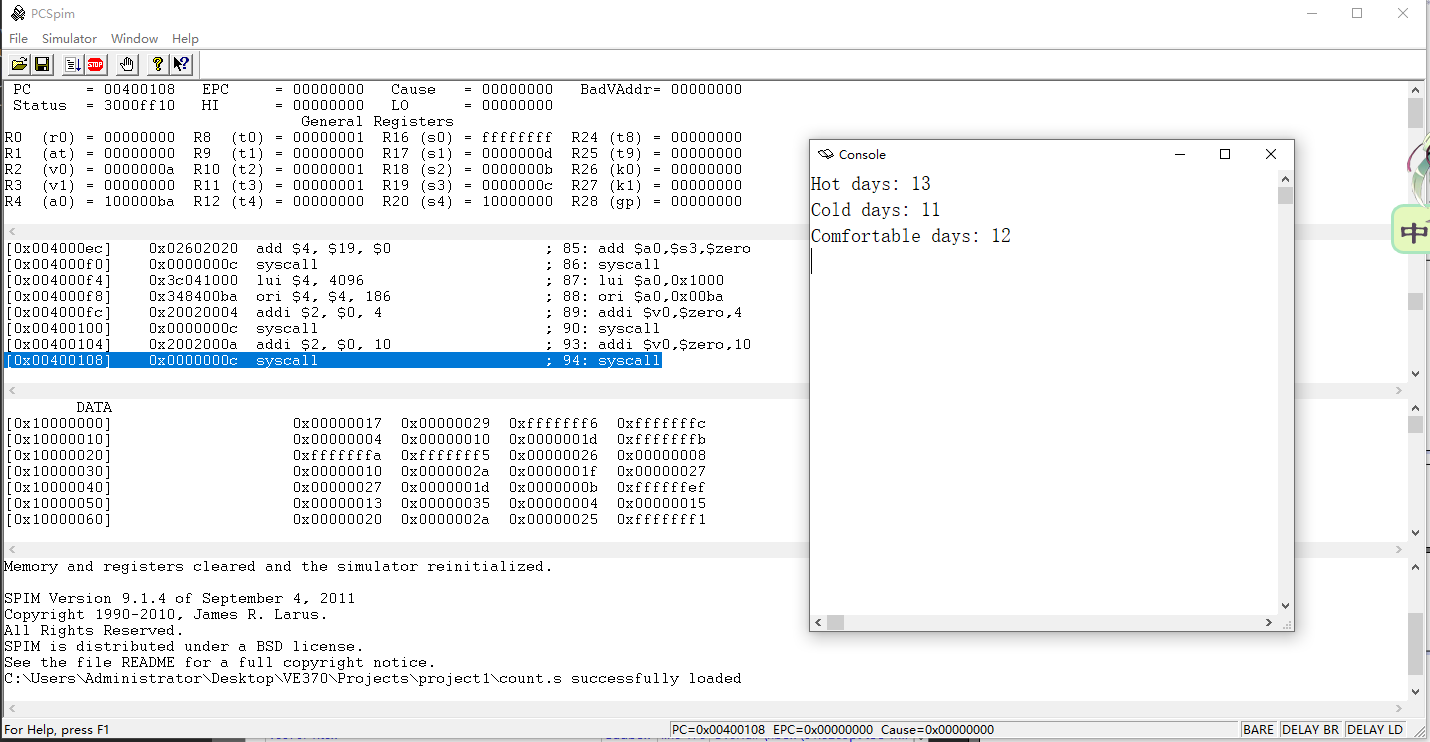
\includegraphics[scale=0.4]{result.png}
\caption{Simulation result}
\label{result}
\end{figure}

\section{Discussion}
\subsection{Input}
\par In order to avoid pushing the array elements into the stack one after another by hand, like the following

\begin{lstlisting}
        sw   $a0, 24($sp)
        addi  $a0, $zero,  7
\end{lstlisting}

I use .word to save the data in the memory. 

\begin{lstlisting}
tempArray: .word 23,41,-10,-4,4,16,29,-5,-6,-11,38,8,16,42,31,39,
39,29,11,-17,19,53,4,21,32,42,37,-15,38,-5,32,-1,41,14,13,18
\end{lstlisting}
By checking the Data block, I found the base address is 0x10000000, which is also shown in Fig \ref{result} above.

\section{Output}
\par To clearly convey what the three outputs indicate, I add a string before each output number, and separate them into three lines. What I need to display is first a string, with terminating symbol, then the number, third the breaking line symbol.
\par To output a string with terminating symbol, I use .asciiz, which means a string ended by an empty character. This could avoid displaying all the characters stored right after. 
\begin{lstlisting}
$output_hot: .asciiz "Hot days: " #90-9a
$output_cold: .asciiz "Cold days: " #9b-a6
$output_comfort: .asciiz "Comfortable days: " #a7-ba
\end{lstlisting}
And by commenting all of them and them uncommented one by one, I found their addresses, which is shown in Fig\ref{straddr}, from 0x10000090 to 0x100000b9
\begin{figure}[H]
\centering
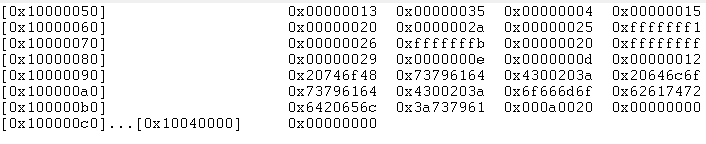
\includegraphics[scale=0.7]{stringadd.png}
\caption{string addresses}
\label{straddr}
\end{figure}

\par To output the number, its just simply syscall.
\par To output the breaking line symbol, I stored "$\backslash$n" character, and found its address to be 0x100000ba. I add one after each number is displayed.

\par A sample output procedure code is shown below
\begin{lstlisting}
    lui $a0,0x1000
    ori $a0,0x0090
    addi $v0,$zero,4
    syscall
    addi $v0,$zero,1
    add $a0,$s1,$zero
    syscall
    lui $a0,0x1000
    ori $a0,0x00ba
    addi $v0,$zero,4
    syscall #display "Hot days: xx \n"
\end{lstlisting}

\subsection{Delay}
\par A damn clever guy posted that the operating sequence is not explicit after jal,j and beq instructions. Therefore we had to add delay right after them in case the program execute some instructions in advance undesirably. The most direct way is nop instruction, but its forbidden in this project.
\subsection{Others}
\par After finishing the project, I get the answer to the question 'where should we push and destroy the stack'. For me, the most wise way is to finish them in the caller, right before and after calling the subfunctions. The reason for not doing these within the subfunctions are: First, we don't know what we should preserve and restore for the caller when writing subfunctions. Second, if we have many multiple subfuncitons to call, pushing and destroying stack within caller function may reduce redundant stack operations, thus the speed is improved.
\par In this project, many functions are actually limited. For example, the pesudo instruction are not allowed. This caused me some trouble when dealing with strings and arrays. If there's no limits, I can simply write
\begin{lstlisting}
output_hot: .asciiz "Hot days: " 
la $a0, output_hot
addi $v0,$zero,4
syscall
\end{lstlisting}
instead of looking for the physical address in the PCspim simulator.
\par Also, I tried using macro, but it seems not available neither.

\section{Appendix}
\begin{lstlisting}
.data
tempArray: .word 23,41,-10,-4,4,16,29,-5,-6,-11,38,8,16,42,31,39,
39,29,11,-17,19,53,4,21,32,42,37,-15,38,-5,32,-1,41,14,13,18
$output_hot: .asciiz "Hot days: " #90-9a
$output_cold: .asciiz "Cold days: " #9b-a6
$output_comfort: .asciiz "Comfortable days: " #a7-b9
$newline: .asciiz"\n"


.text 
.globl __start

#.macro print_int($int)
#addi $v0,$zero,1
#add $a0,$int,$zero
#syscall
#.end_macro

__start:
#size=s0,hotDay=s1,coldDay=s2,comfortDay=s3,tempArray=s4
    lui $s4,0x1000
    ori $s4,0x0000
    addi $s0,$zero,36
    addi $sp,$sp,-40
    sw $s0,36($sp)
    sw $s1,32($sp)
    sw $s2,28($sp)
    sw $s3,24($sp)
    sw $s4,20($sp)
    add $a0,$s4,$zero
    add $a1,$s0,$zero
    addi $a2,$zero,1
    jal countArray
    add $t7,$t7,$zero

    add $s1,$v0,$zero
    sw $s1,32($sp)
    lw $a0,20($sp)
    lw $a1,36($sp)
    addi $a2,$zero,-1
    jal countArray
    add $t7,$t7,$zero

    add $s2,$v0,$zero
    sw $s2,28($sp)
    lw $a0,20($sp)
    lw $a1,36($sp)
    add $a2,$zero,$zero
    jal countArray
    add $t7,$t7,$zero

    add $s3,$v0,$zero
    lw $s1,32($sp)
    lw $s2,28($sp)
    addi $sp,$sp,40

    lui $a0,0x1000
    ori $a0,0x0090
    addi $v0,$zero,4
    syscall
    addi $v0,$zero,1
    add $a0,$s1,$zero
    syscall
    lui $a0,0x1000
    ori $a0,0x00ba
    addi $v0,$zero,4
    syscall #display "Hot days: xx \n"

    lui $a0,0x1000
    ori $a0,0x009b
    addi $v0,$zero,4
    syscall
    addi $v0,$zero,1
    add $a0,$s2,$zero
    syscall
    lui $a0,0x1000
    ori $a0,0x00ba
    addi $v0,$zero,4
    syscall

    lui $a0,0x1000
    ori $a0,0x00a7
    addi $v0,$zero,4
    syscall
    addi $v0,$zero,1
    add $a0,$s3,$zero
    syscall
    lui $a0,0x1000
    ori $a0,0x00ba
    addi $v0,$zero,4
    syscall
#print

    addi $v0,$zero,10
    syscall

#countArray***************************************
countArray:
    addi $s0,$a1,-1  # i=s0, i initilaized to be numElements-1
    add $s1,$zero,$zero  #s1=cnt=0
    j For
    add $t7,$t7,$zero

For:
    slt $t0,$s0,$zero #s0<0?
    addi $t2,$zero,1
    beq $t0,$t2,ExitFor
    add $t7,$t7,$zero    
    
    #stack
    addi $sp,$sp,-32
    sw $a0,28($sp)
    sw $a1,24($sp)
    sw $a2,20($sp)
    sw $s0,16($sp)
    sw $s1,12($sp)
    sw $ra,8($sp)
    add $s2,$a0,$zero  #s2=A[]
    sll $t0,$s0,2
    add $s2,$s2,$t0

    addi $t2,$zero,1
    beq $a2,$t2,Hotplus
    addi $t2,$zero,-1
    beq $a2,$t2,Coldplus
    j Comfortplus
    add $t7,$t7,$zero

Hotplus:
    lw $a0,0($s2)
    jal Hot 
    add $t7,$t7,$zero
    j Fortail
    add $t7,$t7,$zero

Coldplus:
    lw $a0,0($s2)
    jal Cold
    add $t7,$t7,$zero
    j Fortail
    add $t7,$t7,$zero

Comfortplus:
    lw $a0,0($s2)
    jal Comfort
    add $t7,$t7,$zero
    j Fortail
    add $t7,$t7,$zero

Fortail:
    lw $a0,28($sp)
    lw $a1,24($sp)
    lw $a2,20($sp)
    lw $s0,16($sp)
    lw $s1,12($sp)
    lw $ra,8($sp)
    add $sp,$sp,32
    add$s1,$s1,$v0
    addi $s0,$s0,-1
    j For
    add $t7,$t7,$zero

ExitFor:
    add $v0,$s1,$zero
    jr $ra
    add $t7,$t7,$zero
    #countArray over
    
#**********************************************

Hot:
    addi $t2,$zero,30
    slt $t0,$t2,$a0
    addi $t3,$zero,1
    beq $t0,$t3,hotreturn1
    add $v0,$zero,$zero
    jr $ra
    add $t7,$t7,$zero
    hotreturn1: # greater than 30,hot
        addi $v0,$zero,1
        jr $ra
        add $t7,$t7,$zero

Cold:
    addi $t2,$zero,5
    slt $t0,$t2,$a0
    addi $t3,$zero,1
    beq $t0,$t3,coldreturn0
    addi $v0,$zero,1
    jr $ra
    add $t7,$t7,$zero
    coldreturn0: #greater than 5, not cold
        add $v0,$zero,$zero
        jr $ra
        add $t7,$t7,$zero

Comfort:
    addi $t2,$zero,30
    slt $t0,$t2,$a0
    addi $t3,$zero,1
    beq $t0,$t3,comfortreturn0   
    addi $t2,$zero,5
    slt $t0,$a0,$t2
    beq $t0,$t3,comfortreturn0 
    addi $v0,$zero,1
    jr $ra
    add $t7,$t7,$zero
    comfortreturn0:
        add $v0,$zero,$zero
        jr $ra
        add $t7,$t7,$zero
\end{lstlisting}
\end{document}